\documentclass[a4paper,12pt,reqno]{article}

% --------------------------------------------------------
% Packages
% --------------------------------------------------------
\usepackage[utf8]{inputenc}
\usepackage{mathtools,graphicx}
\usepackage[colorlinks=true, allcolors=blue]{hyperref}
\usepackage{amsmath,amsfonts,amssymb,amsthm,mathrsfs,bm}
\usepackage[margin=0.95in]{geometry}
\usepackage{setspace}
\usepackage[table,xcdraw]{xcolor}
\usepackage{float} % 支持图片浮点嵌入 e.g.,\begin{figure}[H]
\usepackage{subfigure} % 支持多图
\usepackage{cite}
\usepackage{siunitx} % 支持各类正体单位 e.g.,\unit{\kg}(建议在数字和单位间插入\,以留出适当间隙)
\usepackage{txfonts} % 支持正体希腊字母 e.g.,$\muup$ 注:添加该包会对默认字体有影响
\usepackage{url} % bibTex支持引用网页

% --------------------------------------------------------
% Custom Commands
% --------------------------------------------------------
% \renewcommand{\rmdefault}{phv} % Arial
% \renewcommand{\sfdefault}{phv} % Arial
\renewcommand\thesection{\arabic {section}} % Section numbers start from 1
% \renewcommand{\bibname}{References}
\newcommand{\HRule}{\rule{\linewidth}{0.5mm}}
\DeclareUnicodeCharacter{2212}{-}

% --------------------------------------------------------
% Opening: Title and Author Names
% --------------------------------------------------------
\begin{document}

\textsc{
    \vspace{-3cm}
    \begin{center}
        \center\LARGE Queen's University Belfast \\[0.5cm]
        \Large ELE8096 Wireless Sensor Systems \\[0.5cm]
    \end{center} 
}
\textsc{
    % \vspace{-1cm}
    \begin{flushleft}
        \Large Coursework1 \hfill
        % \small Student: \ \ \ \ \ \ Zichi Zhang \ Student Number: 40299571\\
        % \hfill Muzixiang Xiao \, \ \ \ \ \ \ \ \ \ \ \ \ \ \ \ \ \ \ \ \ \ \ \ \ \ \ \ \ \ 40344034\\
        % \hfill Jiyu Zou \, \ \ \ \ \ \ \ \ \ \ \ \ \ \ \ \ \ \ \ \ \ \ \ \ \ \ \ \ \ 40344034\\
        % \hfill Yuhang Zhang \, \ \ \ \ \ \ \ \ \ \ \ \ \ \ \ \ \ \ \ \ \ \ \ \ \ \ \ \ \ 40344034\\
        % \hfill Chuao Zheng \, \ \ \ \ \ \ \ \ \ \ \ \ \ \ \ \ \ \ \ \ \ \ \ \ \ \ \ \ \ 40344034\\
        % \hfill Yujie Yang \, \ \ \ \ \ \ \ \ \ \ \ \ \ \ \ \ \ \ \ \ \ \ \ \ \ \ \ \ \ 40344034
        \large Group: 5
    \end{flushleft}
}

% --------------------------------------------------------
% Section 1: Group Task – Data Set and Basic Statistics
% --------------------------------------------------------
\vspace{-0.5cm}
\section*{Part II: Group Task – Data Set and Basic Statistics}\label{sec:1}

% Subsection: Identifying a Data Set
% ^^^^^^^^^^^^^^^^^^^^^^^^^^^
\vspace{-0.2cm}
\subsection*{Identifying a Data Set}
    We build a Github Repositorie and upload the data set, it is public to check from this link:
    \href{https://github.com/Gczmy/ELE8096/blob/main/Coursework1_Group_Part/NO2_DATA.xlsx}{The Data Set}. 
    And the data source is from the UK AIR Air Information Resource, it can be check with some steps from this link:
    \href{https://uk-air.defra.gov.uk/data/datawarehouse}{The Data Source}.\\

% Subsection: Background on the importance of pollutant and legislation on thresholds
% ^^^^^^^^^^^^^^^^^^^^^^^^^^^
\vspace{-0.5cm}
\subsection*{Background on the importance of pollutant and legislation on thresholds}
    Nitrogen Dioxide (NO$_2$) is one of a group of 
    highly reactive gases known as oxides of nitrogen 
    or nitrogen oxides (NO$_{\mathrm{x}}$). Other 
    nitrogen oxides include nitrous acid and nitric 
    acid. NO$_2$ is used as the indicator for the 
    larger group of nitrogen oxides \cite{Basic_Information_about_NO2}. 
    \paragraph{The main source of NO$_2$:}
    NO$_2$ primarily gets in the air from the burning of fuel. 
    NO$_2$ forms from emissions from cars, trucks and buses, 
    power plants, and off-road equipment.Nitrogen 
    dioxide by anthropogenic is mainly released 
    from high-temperature combustion processes, such as 
    motor vehicle exhaust and boiler exhaust emissions. 
    NO$_2$ is mainly derived from the oxidation of NO, producing 
    approximately $568\times106$ tons per year. The various nitrogen 
    oxides emitted by human activities mainly come from the 
    combustion process of various fuels, among which industrial 
    kilns and automobiles are the most important. 
    NO$_{\mathrm{x}}$ generation 
    pathway during fuel combustion: Nitrogen in the air is 
    oxidized at high temperature. The NO$_{\mathrm{x}}$ 
    generated in this way 
    is called thermally induced NO$_{\mathrm{x}}$. 
    The amount of NO$_{\mathrm{x}}$ generated 
    is a function of flame structure and temperature. The 
    higher the temperature, the greater the concentration of 
    oxygen in the combustion zone, and the greater the amount 
    of NO$_{\mathrm{x}}$ produced \cite{Baidu_oxides}.
    \paragraph{Health effects of NO$_2$:}
    Breathing air with a high concentration of NO$_2$ can 
    irritate airways in the human respiratory system. Such 
    exposures over short periods can aggravate respiratory 
    diseases, particularly asthma, leading to respiratory 
    symptoms (such as coughing, wheezing or difficulty 
    breathing), hospital admissions and visits to emergency 
    rooms. Longer exposures to elevated concentrations of 
    NO$_2$ may contribute to the development of asthma and 
    potentially increase susceptibility to respiratory 
    infections. People with asthma, as well as children and 
    the elderly are generally at greater risk for  the 
    health effects of NO$_2$.
    NO$_2$ along with other NO$_{\mathrm{x}}$ reacts with 
    other chemicals in the air to form both particulate 
    matter and ozone. Both of these are also harmful when 
    inhaled due to effects on the respiratory system.\\
    Nitrogen dioxide is one of the causes of acid rain 
    and has a variety of environmental effects, including 
    effects on competition and changes in composition 
    between wetland and terrestrial plant species, 
    reduced atmospheric visibility, acidification of 
    surface water, eutrophication (lack of oxygen due 
    to algal blooms rich in nutrients such as nitrogen 
    and phosphorus in the water) and increased levels 
    of toxins in the water column that are harmful to 
    fish and other aquatic organisms \cite{Baidu_nitrogen}.

% Subsection: Basic statistics on the data set
% ^^^^^^^^^^^^^^^^^^^^^^^^^^^
\vspace{-0.5cm}
\subsection*{Basic statistics on the data set}
    \subsubsection*{12 months average duiring this year}
        The figures of 12 months average duiring this year is shown below 
        as Figure \ref{fig:12_months_average_duiring_this_year}.\\
        The Figure \ref{fig:12_months_average_duiring_this_year} shows the variation of Nitrogen dioxide (NO$_2$) 
        concentration during Dec 2020 to Nov 2021. It is obvious 
        that the graph keeps fluctuating from the end of Dec 2020 
        to the beginning of Sep 2021 in the range of about 38\,\si{\ug/\m^3} 
        to 22\,\si{\ug/\m^3}. Then a significant drop of NO$_2$ is illustrated 
        from Sep 2021 to Oct 2021, following a similar magnitude of 
        increasing of that until the beginning of Nov 2021. \\
        As mentioned above, the NO$_2$ mainly be produced through the 
        gas released from vehicle and charcoal burning for heating. 
        Then, the ascending trend from Dec 2020 to Jan 2021 and 
        Oct 2021 to Nov 2021 could be explained as the demand of 
        heat increased due to the approaching of winter. For the 
        descending trend from Sep 2021 to Oct 2021, a possible 
        explanation could be the strike of lorry drivers during 
        this period \cite{Gareth}, their strike leads to decreasing of 
        vehicle tail gas. Despite that, the average value of NO$_2$ 
        concentration in the air is about 30 in approximation.
        \begin{figure}[H]
            \centering
            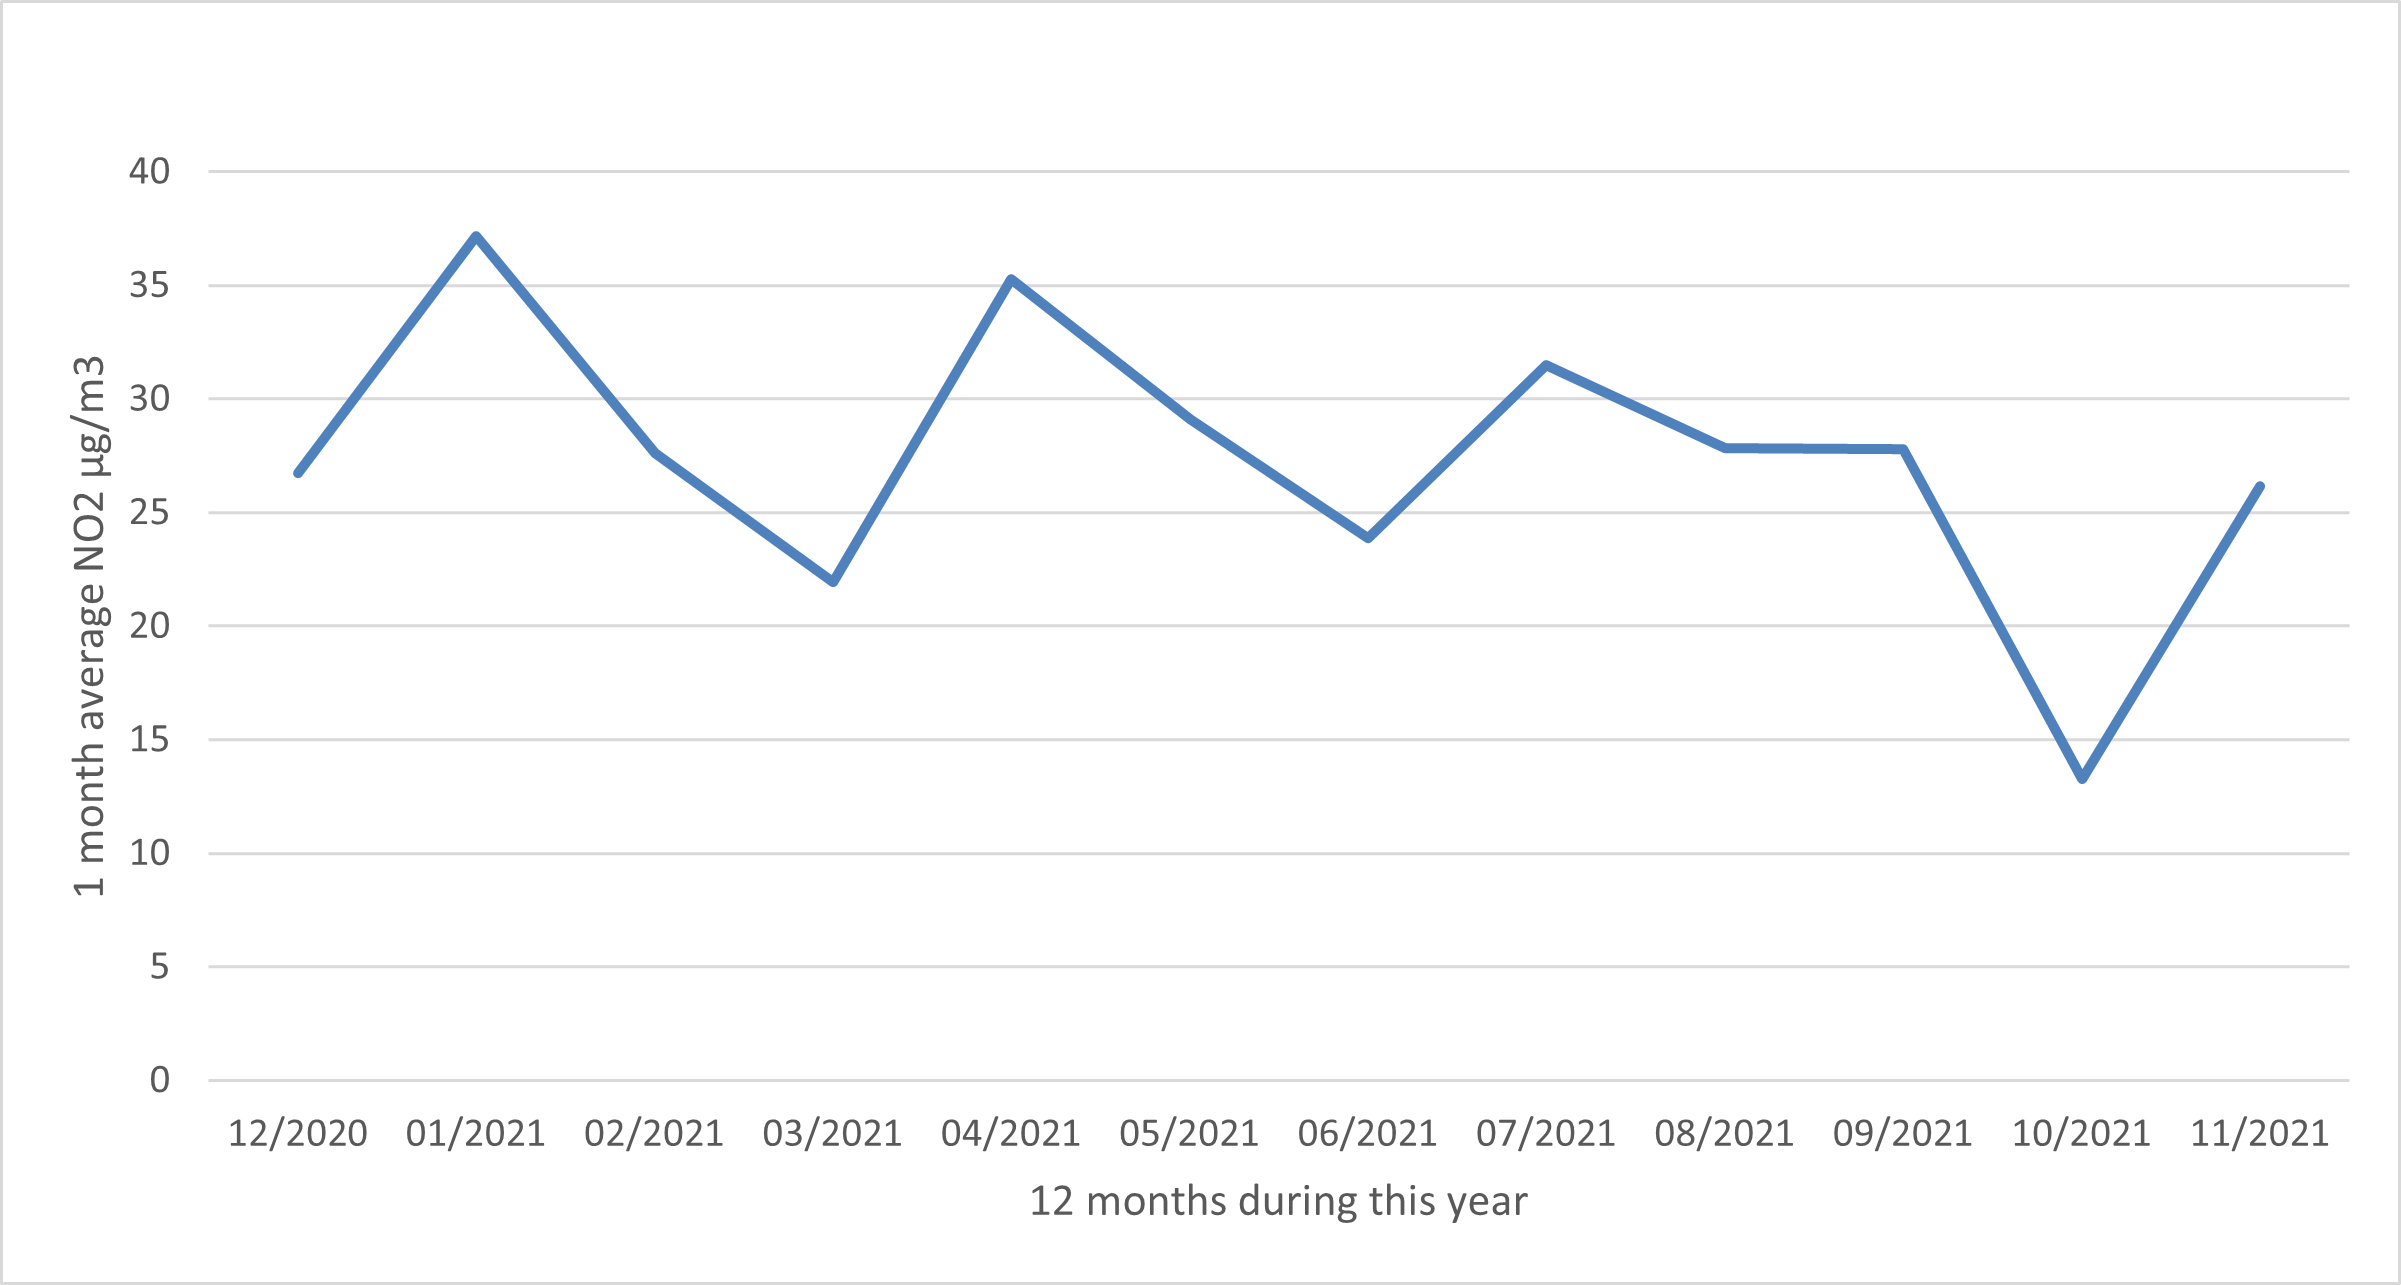
\includegraphics[width=0.7\textwidth]{figures/figure1.png}
            \caption{12 months average duiring this year}
            \label{fig:12_months_average_duiring_this_year}
        \end{figure}
         
    \subsubsection*{4 season 15th comparison}
        The figures of 4 season 15th comparison is shown below 
        as Figure \ref{fig:4_season_15th_comparison}.\\
        The Figure \ref{fig:4_season_15th_comparison} shows the nitrogen 
        dioxide concentration comparison on January 15th, April 15th, 
        July 15th and October 15th. Because of the winter central heating, 
        the night’s nitrogen dioxide concentration in January and April 
        is significantly higher than the same time in July and October. 
        Motor vehicle emissions is the mainly reason why the nitrogen 
        dioxide concentration is the highest from 7:00 to 10:00 in January 
        and April. Paradoxically, overall nitrogen dioxide concentration 
        were the lowest in October. One of the main reason is truckers 
        strike in Britain.
        \begin{figure}[H]
            \centering
            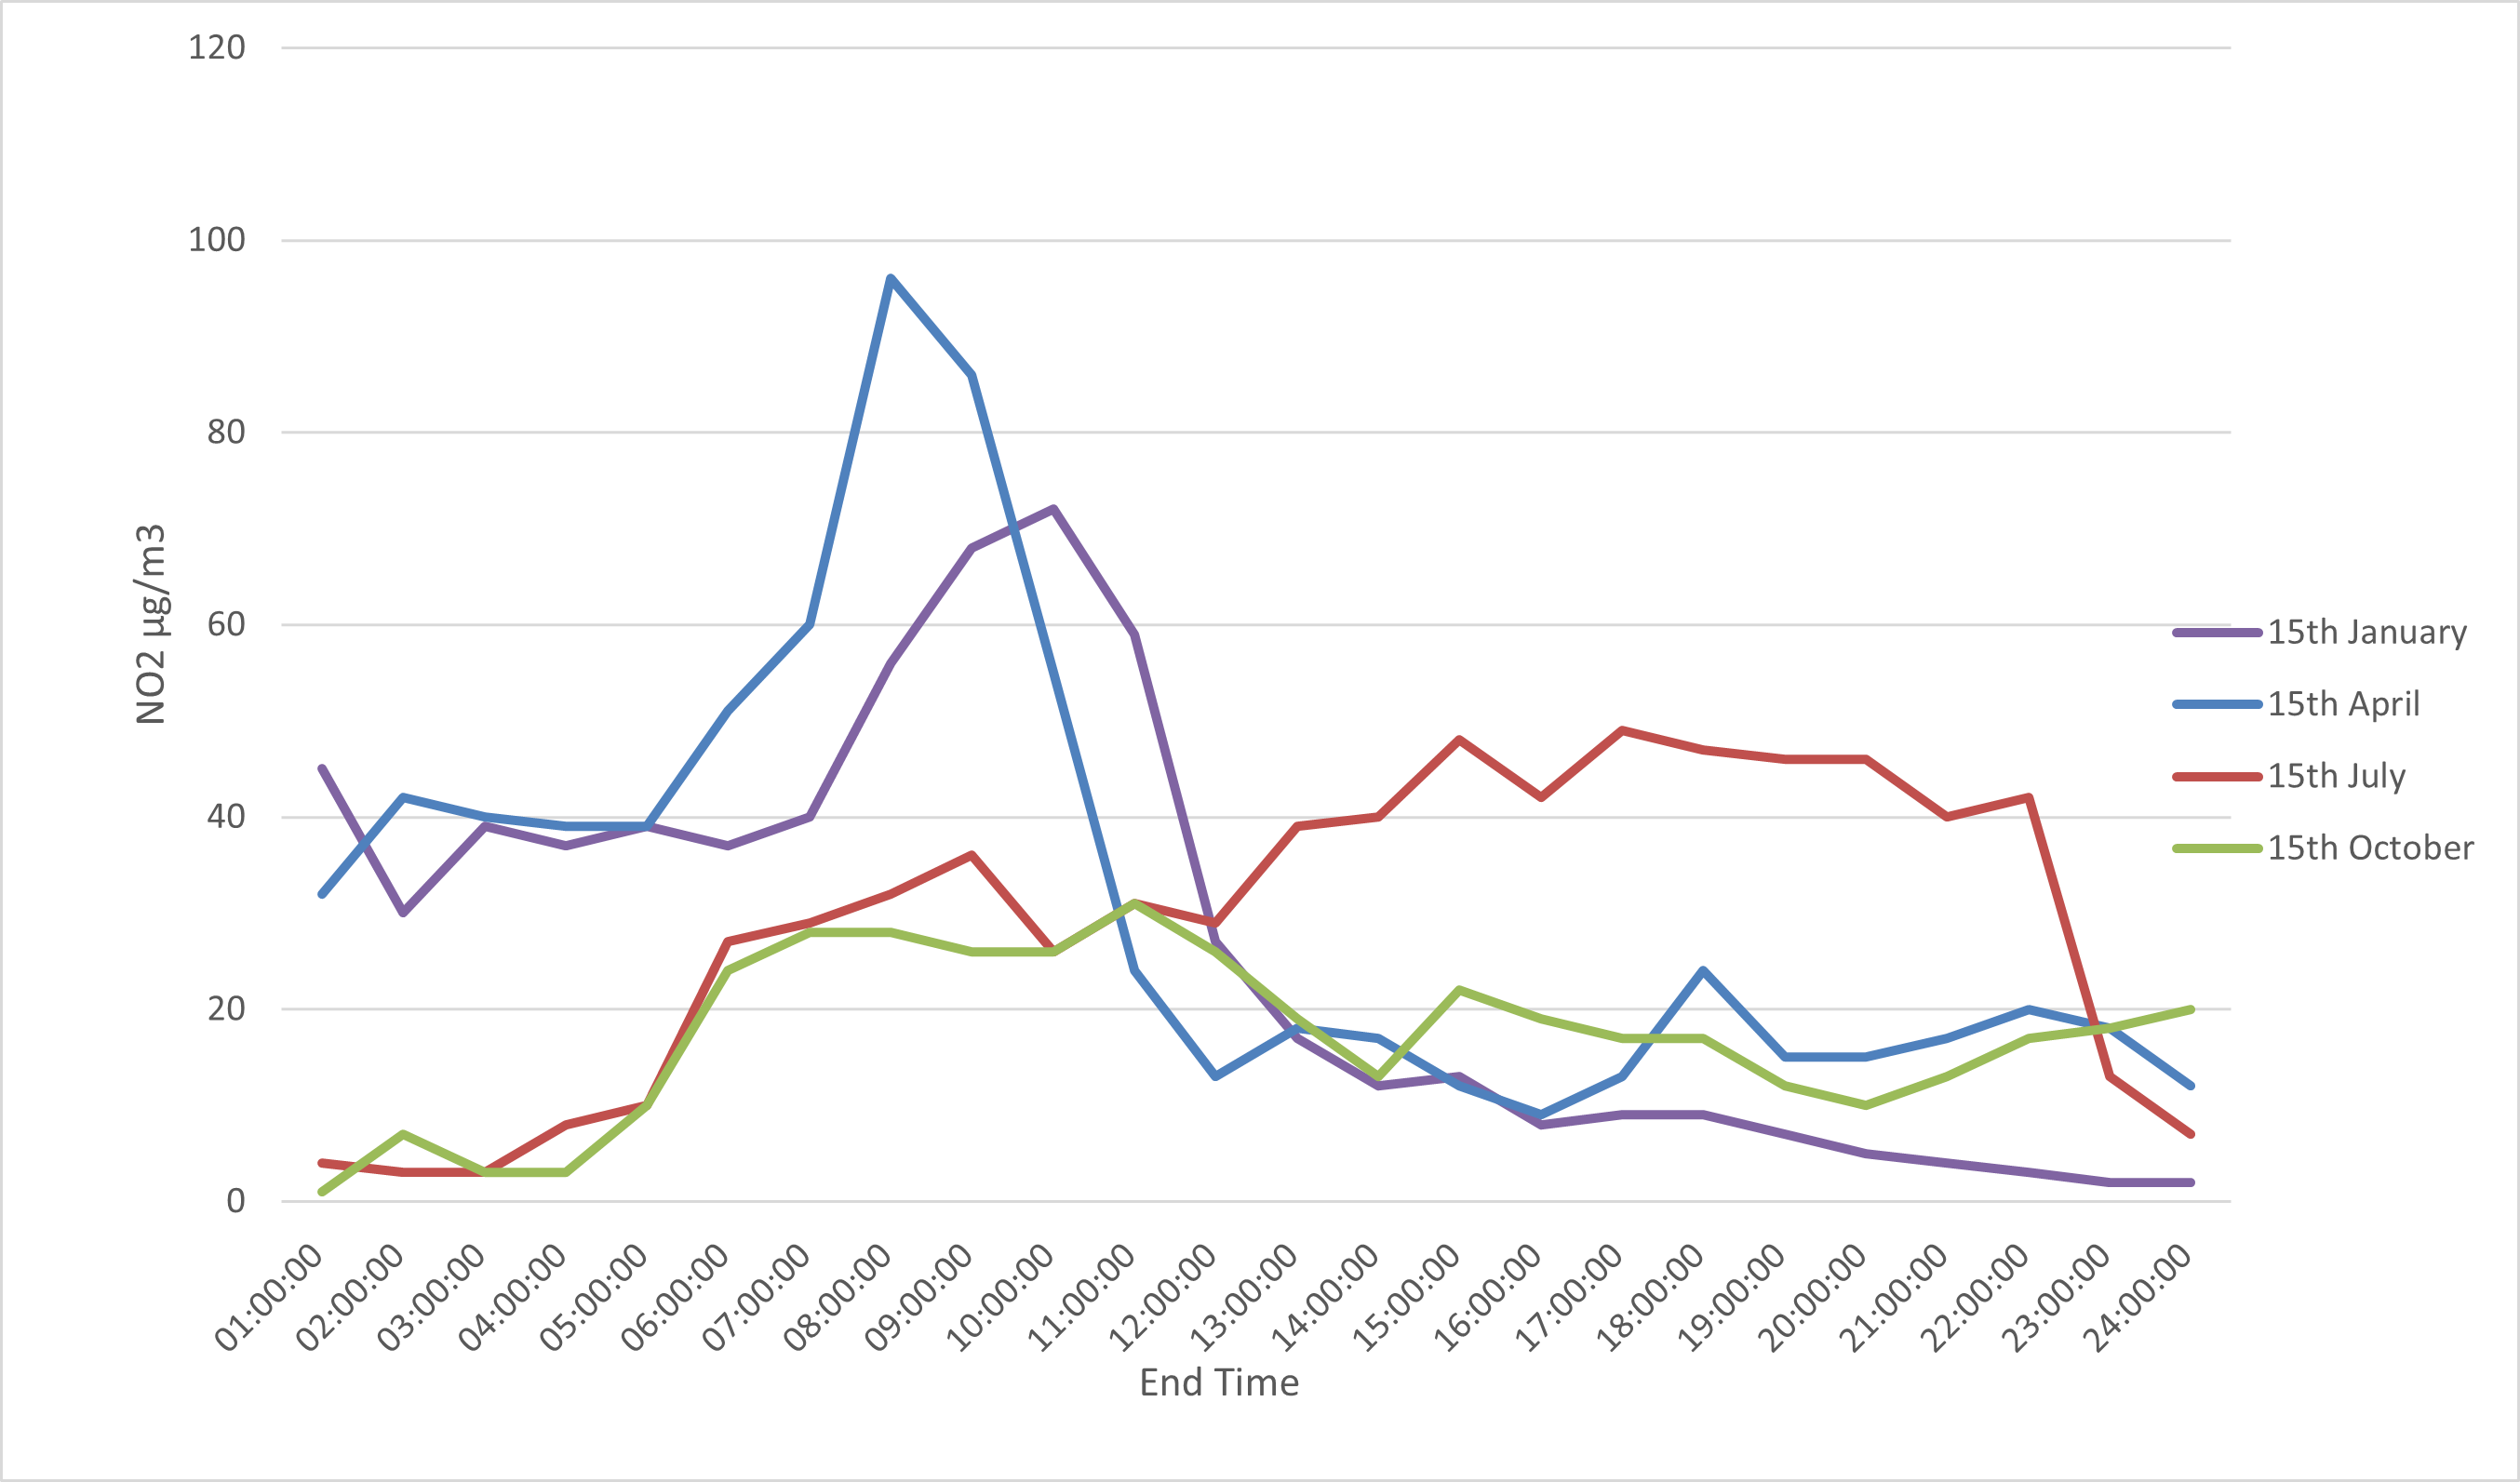
\includegraphics[width=0.7\textwidth]{figures/figure2.png}
            \caption{4 season 15th comparison}
            \label{fig:4_season_15th_comparison}
        \end{figure}
        

\newpage

\bibliographystyle{IEEEtran}
\bibliography{References}
\end{document}
